\documentclass[notes]{beamer}

\title{Mesos}
\author{Michael Whittaker}

\usepackage{etoolbox}
\usepackage{external}
\usepackage{hyperref}
\usepackage{slides}

\usepackage{tikz}
\usetikzlibrary{decorations.pathmorphing}
\usetikzlibrary{decorations.pathreplacing}
\usetikzlibrary{patterns}
\usetikzlibrary{shapes}

\newcommand{\smallnote}[1]{\note{\tiny #1}}

\begin{document}

\begin{frame}
  
\includegraphics[width=\textwidth]{mesos-logo.png}

  \begin{center}
    Michael Whittaker
  \end{center}

  \smallnote{
    I'm Michael, and I'll be presenting Mesos: a distributed two-level cluster
    scheduler.
  }
\end{frame}

%%%%%%%%%%%%%%%%%%%%%%%%%%%%%%%%%%%%%%%%%%%%%%%%%%%%%%%%%%%%%%%%%%%%%%%%%%%%%%%%
% Overview
%%%%%%%%%%%%%%%%%%%%%%%%%%%%%%%%%%%%%%%%%%%%%%%%%%%%%%%%%%%%%%%%%%%%%%%%%%%%%%%%
\tikzstyle{server}=[inner sep=0, outer sep=0]
\tikzstyle{slot}=[draw, opacity=0.8, minimum width=0.9cm, minimum height=0.4cm]
\tikzstyle{framework}=[draw, minimum width=2cm, minimum height=1cm]
\tikzstyle{frameworktwo}=[draw, minimum width=2cm, minimum height=2.5cm]

\newcommand{\red}{red!50}
\newcommand{\orange}{orange!50}
\newcommand{\green}{green!50}
\newcommand{\blue}{blue!50}
\newcommand{\purple}{purple!50}
\newcommand{\black}{black!50}

\newcommand{\boundingbox}{
  % \draw[help lines] (0, 0) grid (8.5, 7);
  \path (0, -1) grid (8.5, 7);
}

% \drawserver
%   1: {id}
%   2: {x-coordinate}
%   3: {y-coordinate}
\newcommand{\drawserver}[3]{
  \node[server] (s#1) at (#2, #3) {
\includegraphics[width=1cm]{server.png}};
}

% \drawslots
%   1: {id}
%   2: {x-coordinate}
%   3: {y-coordinate}
%   4: {slot 0 color}
%   5: {slot 1 color}
%   6: {slot 2 color}
\newcommand{\drawslots}[6]{
  \drawserver{#1}{#2}{#3};
  \node[slot, fill=#4] (s#1.0) at (#2, #3+0.5) {};
  \node[slot, fill=#5] (s#1.1) at (#2, #3    ) {};
  \node[slot, fill=#6] (s#1.2) at (#2, #3-0.5) {};
}

% \oneslot{x}{y}{color}
\newcommand{\oneslot}[3]{
  \draw[fill=#3] (#1, #2) rectangle (#1 + 0.4, #2 + 0.9);
}

% \twoslots{x}{y}{color 1}{color 2}
\newcommand{\twoslots}[4]{
  \oneslot{#1}{#2}{#3}
  \oneslot{#1 + 0.5}{#2}{#4}
}

% \threeslots{x}{y}{color 1}{color 2}{color 3}
\newcommand{\threeslots}[5]{
  \oneslot{#1}{#2}{#3}
  \oneslot{#1 + 0.5}{#2}{#4}
  \oneslot{#1 + 1.0}{#2}{#5}
}

% \fourslots{x}{y}{color 1}{color 2}{color 3}{color 4}
\newcommand{\fourslots}[6]{
  \oneslot{#1}{#2}{#3}
  \oneslot{#1 + 0.5}{#2}{#4}
  \oneslot{#1 + 1.0}{#2}{#5}
  \oneslot{#1 + 1.5}{#2}{#6}
}

\newcommand{\hadoopone}{
  \node[
    draw,
    minimum width=5cm, minimum height=3cm,
    label={[shift={(0, -1cm)}]north:Hadoop}
  ] (hadoop) at (5, 4.5) {};
  \foreach \i in {0, ..., 5} {
    \draw (hadoop) -- (s\i);
  }
}

\newcommand{\hadooptwo}{
  \node[
    draw,
    minimum width=5cm, minimum height=3cm,
    label={[shift={(0, -1cm)}]north:Hadoop}
  ] (hadoop) at (2, 4.5) {};
}

\newcommand{\stormtwo}{
  \node[
    draw,
    minimum width=5cm, minimum height=3cm,
    label={[shift={(0, -1cm)}]north:Storm}
  ] (storm) at (8, 4.5) {};
}

\newcommand{\hadooptwofull}{
  \hadooptwo{}
  \foreach \i in {0, ..., 2} {
    \draw (hadoop) -- (s\i);
  }
}

\newcommand{\stormtwofull}{
  \stormtwo{}
  \foreach \i in {3, ..., 5} {
    \draw (storm) -- (s\i);
  }
}

\newcommand{\tear}{
  \draw[decoration = {zigzag,segment length = 4mm, amplitude = 1mm}, decorate]
    (5, 6.5) -- (5, -1);
}

\begin{frame}
  \smallnote{
    Let's imagine we're running a large company that offers word count as a
    service. Business is booming, so we bought a large cluster of computers.
  }
  \makebox[\textwidth][c]{
    \centering
    \begin{tikzpicture}
      \boundingbox{}

      \drawserver{0}{0 }{0}
      \drawserver{1}{2 }{0}
      \drawserver{2}{4 }{0}
      \drawserver{3}{6 }{0}
      \drawserver{4}{8 }{0}
      \drawserver{5}{10}{0}
    \end{tikzpicture}
  }
\end{frame}

\begin{frame}
  \smallnote{
    Each computer's resources is further divided into slots. For example, if
    each machine had 3 cores and 3 GB of memory, then each slot could be 1 core
    and 1 GB of memory.
  }
  \makebox[\textwidth][c]{
    \centering
    \begin{tikzpicture}
      \boundingbox{}

      \drawslots{0}{0 }{0}{white}{white}{white}
      \drawslots{1}{2 }{0}{white}{white}{white}
      \drawslots{2}{4 }{0}{white}{white}{white}
      \drawslots{3}{6 }{0}{white}{white}{white}
      \drawslots{4}{8 }{0}{white}{white}{white}
      \drawslots{5}{10}{0}{white}{white}{white}
    \end{tikzpicture}
  }
\end{frame}

\begin{frame}
  \smallnote{
    As a word counting company, of course, we want to run Hadoop on this
    cluster.
  }
  \makebox[\textwidth][c]{
    \centering
    \begin{tikzpicture}
      \boundingbox{}

      \hadoopone{}

      \drawslots{0}{0 }{0}{white}{white}{white}
      \drawslots{1}{2 }{0}{white}{white}{white}
      \drawslots{2}{4 }{0}{white}{white}{white}
      \drawslots{3}{6 }{0}{white}{white}{white}
      \drawslots{4}{8 }{0}{white}{white}{white}
      \drawslots{5}{10}{0}{white}{white}{white}
    \end{tikzpicture}
  }
\end{frame}

\begin{frame}
  \smallnote{
    Users submit tasks to Hadoop which I'm representing here as these colored
    rectangles. For example, these red tasks could be map tasks, these blue
    tasks could be reduce tasks, and so on.
  }
  \makebox[\textwidth][c]{
    \centering
    \begin{tikzpicture}
      \boundingbox{}

      \hadoopone{}
      \fourslots{3}{3.5}{\red}{\red}{\blue}{\blue}
      \fourslots{5}{3.5}{\green}{\green}{\orange}{\orange}

      \drawslots{0}{0 }{0}{white}{white}{white}
      \drawslots{1}{2 }{0}{white}{white}{white}
      \drawslots{2}{4 }{0}{white}{white}{white}
      \drawslots{3}{6 }{0}{white}{white}{white}
      \drawslots{4}{8 }{0}{white}{white}{white}
      \drawslots{5}{10}{0}{white}{white}{white}
    \end{tikzpicture}
  }
\end{frame}

\begin{frame}
  \smallnote{
    Hadoop has full control over the cluster and starts scheduling the tasks
    into the machine's slots. Here, it scheduled the first task on the first
    machine.
  }
  \makebox[\textwidth][c]{
    \centering
    \begin{tikzpicture}
      \boundingbox{}

      \hadoopone{}
      \fourslots{3}{3.5}{\red}{\blue}{\blue}{\green}
      \threeslots{5}{3.5}{\green}{\orange}{\orange}

      \drawslots{0}{0 }{0}{\red}{white}{white}
      \drawslots{1}{2 }{0}{white}{white}{white}
      \drawslots{2}{4 }{0}{white}{white}{white}
      \drawslots{3}{6 }{0}{white}{white}{white}
      \drawslots{4}{8 }{0}{white}{white}{white}
      \drawslots{5}{10}{0}{white}{white}{white}
    \end{tikzpicture}
  }
\end{frame}

\begin{frame}
  \smallnote{
    And here, it scheduled the second task on the second machine.
  }
  \makebox[\textwidth][c]{
    \centering
    \begin{tikzpicture}
      \boundingbox{}

      \hadoopone{}
      \fourslots{3}{3.5}{\blue}{\blue}{\green}{\green}
      \twoslots{5}{3.5}{\orange}{\orange}

      \drawslots{0}{0 }{0}{\red}{white}{white}
      \drawslots{1}{2 }{0}{\red}{white}{white}
      \drawslots{2}{4 }{0}{white}{white}{white}
      \drawslots{3}{6 }{0}{white}{white}{white}
      \drawslots{4}{8 }{0}{white}{white}{white}
      \drawslots{5}{10}{0}{white}{white}{white}
    \end{tikzpicture}
  }
\end{frame}

\begin{frame}
  \smallnote{
    Hadoop keeps scheduling tasks...
  }
  \makebox[\textwidth][c]{
    \centering
    \begin{tikzpicture}
      \boundingbox{}

      \hadoopone{}
      \oneslot{3}{3.5}{\orange}

      \drawslots{0}{0 }{0}{\red }{\blue}{white}
      \drawslots{1}{2 }{0}{\red }{\blue}{white}
      \drawslots{2}{4 }{0}{\green}{white}{white}
      \drawslots{3}{6 }{0}{\green}{white}{white}
      \drawslots{4}{8 }{0}{\orange}{white}{white}
      \drawslots{5}{10}{0}{white}{white}{white}
    \end{tikzpicture}
  }
\end{frame}

\begin{frame}
  \smallnote{
    when maybe more tasks arrive.
  }
  \makebox[\textwidth][c]{
    \centering
    \begin{tikzpicture}
      \boundingbox{}

      \hadoopone{}
      \fourslots{3}{3.5}{\orange}{\red}{\green}{\red}
      \fourslots{5}{3.5}{\purple}{\purple}{\black}{\purple}

      \drawslots{0}{0 }{0}{\red }{\blue}{white}
      \drawslots{1}{2 }{0}{\red }{\blue}{white}
      \drawslots{2}{4 }{0}{\green}{white}{white}
      \drawslots{3}{6 }{0}{\green}{white}{white}
      \drawslots{4}{8 }{0}{\orange}{white}{white}
      \drawslots{5}{10}{0}{white}{white}{white}
    \end{tikzpicture}
  }
\end{frame}

\begin{frame}
  \smallnote{
    This is no problem. Hadoop schedules these tasks too. Life is good for our
    word counting business.
  }
  \makebox[\textwidth][c]{
    \centering
    \begin{tikzpicture}
      \boundingbox{}

      \hadoopone{}

      \drawslots{0}{0 }{0}{\red }{\blue}{white}
      \drawslots{1}{2 }{0}{\red }{\blue}{\purple}
      \drawslots{2}{4 }{0}{\green}{\purple}{\black}
      \drawslots{3}{6 }{0}{\green}{\purple}{white}
      \drawslots{4}{8 }{0}{\orange}{\green}{white}
      \drawslots{5}{10}{0}{\red}{\purple}{white}
    \end{tikzpicture}
  }
\end{frame}

\begin{frame}
  \smallnote{
    Now imagine that as our business grows, we want to start doing more
    complicated things. For example, maybe we want to monitor the amount of
    traffic our service is getting and detect when traffic is abnormally high
    or abnormally low. We can perform this anomaly detection using a stream
    processing system like Apache Storm. You could also image that we may want
    to run a production instance of Hadoop alongside a development version of
    Hadoop. Or maybe, we want to run two versions of Hadoop at the same time.
    Or maybe, the latest and greatest data processing framework was just
    released and it is really good at handling a specific type of application.
    Whatever the reasons, the question arises, how do we divide the cluster
    between these two frameworks?
  }
  \makebox[\textwidth][c]{
    \centering
    \begin{tikzpicture}
      \boundingbox{}

      \hadooptwo{}
      \stormtwo{}

      \drawslots{0}{0 }{0}{white}{white}{white}
      \drawslots{1}{2 }{0}{white}{white}{white}
      \drawslots{2}{4 }{0}{white}{white}{white}
      \drawslots{3}{6 }{0}{white}{white}{white}
      \drawslots{4}{8 }{0}{white}{white}{white}
      \drawslots{5}{10}{0}{white}{white}{white}
    \end{tikzpicture}
  }
\end{frame}

\begin{frame}
  \smallnote{
    The most naive way is to simply divide the cluster completely in two.
    Hadoop gets to manage the first three machines and Storm gets to manage the
    last three machines.
  }
  \makebox[\textwidth][c]{
    \centering
    \begin{tikzpicture}
      \boundingbox{}

      \hadooptwofull{}
      \stormtwofull{}
      \tear{}

      \drawslots{0}{0 }{0}{white}{white}{white}
      \drawslots{1}{2 }{0}{white}{white}{white}
      \drawslots{2}{4 }{0}{white}{white}{white}
      \drawslots{3}{6 }{0}{white}{white}{white}
      \drawslots{4}{8 }{0}{white}{white}{white}
      \drawslots{5}{10}{0}{white}{white}{white}
    \end{tikzpicture}
  }
\end{frame}

\begin{frame}
  \smallnote{
    Let's say we go with this model and tasks start flowing in. Hadoop gets a
    lot of tasks to schedule and Storm only gets a handful.
  }
  \makebox[\textwidth][c]{
    \centering
    \begin{tikzpicture}
      \boundingbox{}

      \hadooptwofull{}
      \stormtwofull{}
      \tear{}

      \fourslots{0}{3.5}{\red}{\red}{\red}{\blue}
      \fourslots{2}{3.5}{\orange}{\orange}{\black}{\black}

      \threeslots{6}{3.5}{\purple}{\purple}{\green}

      \drawslots{0}{0 }{0}{white}{white}{white}
      \drawslots{1}{2 }{0}{white}{white}{white}
      \drawslots{2}{4 }{0}{white}{white}{white}
      \drawslots{3}{6 }{0}{white}{white}{white}
      \drawslots{4}{8 }{0}{white}{white}{white}
      \drawslots{5}{10}{0}{white}{white}{white}
    \end{tikzpicture}
  }
\end{frame}

\begin{frame}
  \smallnote{
    The frameworks start scheduling jobs.
  }
  \makebox[\textwidth][c]{
    \centering
    \begin{tikzpicture}
      \boundingbox{}

      \hadooptwofull{}
      \stormtwofull{}
      \tear{}

      \fourslots{0}{3.5}{\red}{\red}{\blue}{\orange}
      \threeslots{2}{3.5}{\orange}{\black}{\black}

      \twoslots{6}{3.5}{\purple}{\green}

      \drawslots{0}{0 }{0}{\red}{white}{white}
      \drawslots{1}{2 }{0}{white}{white}{white}
      \drawslots{2}{4 }{0}{white}{white}{white}
      \drawslots{3}{6 }{0}{\purple}{white}{white}
      \drawslots{4}{8 }{0}{white}{white}{white}
      \drawslots{5}{10}{0}{white}{white}{white}
    \end{tikzpicture}
  }
\end{frame}

\begin{frame}
  \makebox[\textwidth][c]{
    \centering
    \begin{tikzpicture}
      \boundingbox{}

      \hadooptwofull{}
      \stormtwofull{}
      \tear{}

      \fourslots{0}{3.5}{\red}{\blue}{\orange}{\orange}
      \twoslots{2}{3.5}{\black}{\black}

      \oneslot{6}{3.5}{\green}

      \drawslots{0}{0 }{0}{\red}{white}{white}
      \drawslots{1}{2 }{0}{\red}{white}{white}
      \drawslots{2}{4 }{0}{white}{white}{white}
      \drawslots{3}{6 }{0}{\purple}{white}{white}
      \drawslots{4}{8 }{0}{\purple}{white}{white}
      \drawslots{5}{10}{0}{white}{white}{white}
    \end{tikzpicture}
  }
\end{frame}

\begin{frame}
  \makebox[\textwidth][c]{
    \centering
    \begin{tikzpicture}
      \boundingbox{}

      \hadooptwofull{}
      \stormtwofull{}
      \tear{}

      \fourslots{0}{3.5}{\blue}{\orange}{\orange}{\black}
      \oneslot{2}{3.5}{\black}

      \drawslots{0}{0 }{0}{\red}{white}{white}
      \drawslots{1}{2 }{0}{\red}{white}{white}
      \drawslots{2}{4 }{0}{\red}{white}{white}
      \drawslots{3}{6 }{0}{\purple}{white}{white}
      \drawslots{4}{8 }{0}{\purple}{white}{white}
      \drawslots{5}{10}{0}{\green}{white}{white}
    \end{tikzpicture}
  }
\end{frame}

\begin{frame}
  \smallnote{
    Then maybe a bunch more Hadoop tasks show up, and Storm is still pretty
    lightly loaded.
  }
  \makebox[\textwidth][c]{
    \centering
    \begin{tikzpicture}
      \boundingbox{}

      \hadooptwofull{}
      \stormtwofull{}
      \tear{}

      \fourslots{0}{3.5}{\red}{\red}{\blue}{\orange}
      \fourslots{2}{3.5}{\black}{\black}{\blue}{\blue}

      \oneslot{6}{3.5}{\green}

      \drawslots{0}{0 }{0}{\red}{\blue}{\black}
      \drawslots{1}{2 }{0}{\red}{\orange}{white}
      \drawslots{2}{4 }{0}{\red}{\black}{white}
      \drawslots{3}{6 }{0}{\purple}{white}{white}
      \drawslots{4}{8 }{0}{\purple}{white}{white}
      \drawslots{5}{10}{0}{\green}{white}{white}
    \end{tikzpicture}
  }
\end{frame}

\begin{frame}
  \smallnote{
    Soon, Hadoop runs out of slots and tasks have to be queued up. Meanwhile,
    the Storm side of the cluster has a lot of empty slots in which we could
    run Hadoop tasks. Clearly, statically partitioning the cluster leads to
    very poor cluster utilization. A lot of resources that could be used sit
    idle.  Moreover, imagine these machines are all part of a global file
    system like HDFS or GFS. It might be that a task running on this machine
    needs data stored on this machine. By statically partitioning the cluster,
    we limit the amount of locality our schedulers can take advantage of.
  }
  \makebox[\textwidth][c]{
    \centering
    \begin{tikzpicture}
      \boundingbox{}

      \hadooptwofull{}
      \stormtwofull{}
      \tear{}

      \fourslots{0}{3.5}{\blue}{\orange}{\black}{\black}
      \twoslots{2}{3.5}{\blue}{\blue}

      \drawslots{0}{0 }{0}{\red}{\blue}{\black}
      \drawslots{1}{2 }{0}{\red}{\orange}{\red}
      \drawslots{2}{4 }{0}{\red}{\black}{\red}
      \drawslots{3}{6 }{0}{\purple}{\green}{white}
      \drawslots{4}{8 }{0}{\purple}{white}{white}
      \drawslots{5}{10}{0}{\green}{white}{white}
    \end{tikzpicture}
  }
\end{frame}

\begin{frame}
  \smallnote{
    Clearly, statically partitioning the cluster is a bad idea. Ideally, we'd
    like have a cluster manager which forms a narrow waist between data
    processing frameworks and the underlying cluster.

    We could architect the system to have a single monolithic cluster manager
    that is responsible for scheduling all of the tasks for all of the
    frameworks. Frameworks would communicate their resource requirements,
    location preferences, scheduling preferences, and so on to the cluster
    manager, and the cluster manager would be responsible for scheduling all of
    the tasks. As you read, Borg has this kind of architecture and there are a
    number of advantages. Primarily, the cluster manager has full knowledge of
    the scheduling decisions and can achieve globally optimal scheduling.

    This architecture also has a lot of disadvantages. The cluster manager
    becomes a very complicated piece of software. Different frameworks may
    desire different types of scheduling, so the cluster manager has to support
    a rich set of scheduling policies. The interface between the frameworks and
    the cluster manager has to be flexible enough to support all the existing
    frameworks. And, ...
  }
  \makebox[\textwidth][c]{
    \centering
    \begin{tikzpicture}
      \boundingbox{}

      \node[framework] (Hadoop)  at (0.5, 6) {Hadoop};
      \node[framework] (Storm)   at (3.5, 6) {Storm};
      \node[framework] (Spark)   at (6.5, 6) {Spark};

      \node[
        draw,
        minimum width=5cm, minimum height=2.5cm,
        label={[shift={(0, -1cm)}]north:Monolithic Cluster Manager}
      ] (mesos) at (5, 3) {};
      \foreach \i in {s0, s1, s2, s3, s4, s5, Hadoop, Storm, Spark} {
        \draw (mesos) -- (\i);
      }
      \fourslots{3}{2}{\red}{\red}{\red}{\blue}
      \fourslots{5}{2}{\blue}{\black}{\red}{\black}

      \drawserver{0}{0 }{0}
      \drawserver{1}{2 }{0}
      \drawserver{2}{4 }{0}
      \drawserver{3}{6 }{0}
      \drawserver{4}{8 }{0}
      \drawserver{5}{10}{0}
    \end{tikzpicture}
  }
\end{frame}

\begin{frame}
  \smallnote{
    ...it has to be flexible enough to support all the unknown frameworks that
    haven't yet been developed.
  }
  \makebox[\textwidth][c]{
    \centering
    \begin{tikzpicture}
      \boundingbox{}

      \node[framework] (Hadoop)  at (0.5, 6) {Hadoop};
      \node[framework] (Storm)   at (3.5, 6) {Storm};
      \node[framework] (Spark)   at (6.5, 6) {Spark};
      \node[dashed, framework] (unknown) at (9.5, 6) {???};

      \node[
        draw,
        minimum width=5cm, minimum height=2.5cm,
        label={[shift={(0, -1cm)}]north:Monolithic Cluster Manager}
      ] (mesos) at (5, 3) {};
      \foreach \i in {s0, s1, s2, s3, s4, s5, Hadoop, Storm, Spark} {
        \draw (mesos) -- (\i);
      }
      \draw[dashed] (mesos) -- (unknown);
      \fourslots{3}{2}{\red}{\red}{\red}{\blue}
      \fourslots{5}{2}{\blue}{\black}{\red}{\black}

      \drawserver{0}{0 }{0}
      \drawserver{1}{2 }{0}
      \drawserver{2}{4 }{0}
      \drawserver{3}{6 }{0}
      \drawserver{4}{8 }{0}
      \drawserver{5}{10}{0}
    \end{tikzpicture}
  }
\end{frame}

\begin{frame}
  \smallnote{
    Mesos takes an alternative minimalistic approach and instead pushes
    scheduling decisions into the frameworks. Instead of scheduling all the
    tasks in the system, Mesos simply offers resources to frameworks according
    to some allocation policy and lets the frameworks schedule jobs themselves.
    We'll take a closer look at resource offers soon.

    This two-level scheduling keeps Mesos very simple, very scalable, and
    allows for new data processing frameworks to be developed independently of
    Mesos.
  }
  \makebox[\textwidth][c]{
    \centering
    \begin{tikzpicture}
      \boundingbox{}

      \node[frameworktwo, label={[shift={(0, -1cm)}]north:Hadoop}]
        (Hadoop) at (0.5, 5.5) {};
      \node[frameworktwo, label={[shift={(0, -1cm)}]north:Storm}]
        (Storm) at (3.5, 5.5) {};
      \node[frameworktwo, label={[shift={(0, -1cm)}]north:Spark}]
        (Spark) at (6.5, 5.5) {};
      \node[frameworktwo, dashed, label={[shift={(0, -1cm)}]north:???}]
        (unknown) at (9.5, 5.5) {};

      \threeslots{-0.25}{4.5}{\red}{\red}{\red}
      \threeslots{ 2.75}{4.5}{\blue}{\blue}{\blue}
      \threeslots{ 5.75}{4.5}{\orange}{\orange}{\orange}
      \threeslots{ 8.75}{4.5}{\green}{\green}{\green}

      \node[
        draw,
        minimum width=5cm, minimum height=1cm,
      ] (mesos) at (5, 2.5) {Mesos};
      \foreach \i in {s0, s1, s2, s3, s4, s5, Hadoop, Storm, Spark} {
        \draw (mesos) -- (\i);
      }
      \draw[dashed] (mesos) -- (unknown);

      \drawserver{0}{0 }{0}
      \drawserver{1}{2 }{0}
      \drawserver{2}{4 }{0}
      \drawserver{3}{6 }{0}
      \drawserver{4}{8 }{0}
      \drawserver{5}{10}{0}
    \end{tikzpicture}
  }
\end{frame}

\newcommand{\mesossource}{
  \textcolor{gray}{
    Source: \textit{
      Mesos: A Platform for Fine-Grained Resource Sharing in the Data Center
    }
  }
}

\picframe{mesos-1.pdf}{width=\textwidth}{\mesossource}{
  Now, let's take a closer look at Mesos' architecture with this diagram taken
  from the paper. Mesos consists a of a central master. The master corresponds
  to the Mesos box from the previous slide and is responsible for offering
  resources to frameworks. For fault tolerance, the master has a number of hot
  standbys which use ZooKeeper for leader election when the primary master
  fails. Each machine in the cluster runs a Mesos slave which is responsible
  for reporting available resources to the master and for starting and stopping
  tasks.

  Frameworks plug in to Mesos and have two parts. First, there is the scheduler
  which accepts or rejects resources from the master and oversees the execution
  of its jobs. Second is a framework executor which is launched on each machine
  and executes the jobs.
}

\picframe{mesos-2.pdf}{width=\textwidth}{\mesossource}{
  Resource offers are a key part of Mesos' architecture. Let's walk through the
  example presented in the paper. First, a Mesos slave reports how many
  resources it has available to the Mesos master. Here, slave 1 has 4 CPUs and
  4 GB of RAM. The allocation module of the Mesos master determines how
  resources should be offered. Here, it says to offer all available resources
  to framework 1. Framework 1 responsds to the Mesos master and tells it to run
  two tasks. The first uses 2 CPU and 1 GB of RAM. The second uses 1 CPU and 2
  GB of RAM. The Mesos master forwards the tasks to the slave to be executed by
  the framework's executor. Note that there is still 1 cpu and 1 GB of RAM left
  of the machine. These resources could then be offered to framework 2.

  In this example, the framework accepted the resources offered to it by the
  master, but it doesn't have to. The framework can reject resources it doesn't
  want and wait for resources it does want. For example, if Hadoop wants to run
  a specific map task on a computer which hosts the task's data, it can wait
  for an offer from that computer.
}

\newcommand{\question}[1]{\textcolor{gray}{\textit{Q: #1}}}

\begin{frame}{Resource Allocation}
  \begin{itemize}
    \item
      \question{How are resources offered to frameworks?}
    \item \pause
      A: Pluggable allocation module determines how resources are offered to
      frameworks.

    \item \pause
      \question{When are resources offered to frameworks?}
    \item \pause
      A: Mesos assumes jobs are short and offers resources when tasks end.

    \item \pause
      \question{What if jobs aren't short?}
    \item \pause
      A: Mesos can kill jobs, giving the framework a grace period for cleaning
      up.

    \item \pause
      \question{What if jobs don't want to die?}
    \item \pause
      A: Mesos provides each framework with a guarenteed allocation. So long as
      framework uses less than it's guarenteed allocation, it's jobs won't be
      killed.
  \end{itemize}
\end{frame}


\begin{frame}
  \smallnote{
    Now that we've discussed Mesos' architecture, let's do something fun and
    switch over to a demo. Mesos is now an open source project as part of the
    Apache Software Foundation, so you can actually download and run the code.

    This terminal is SSHed into a virtual machine with 1 CPU and 4 GB of
    memory. This top pane here is running the Mesos master, and this bottom
    pane is running a Mesos slave. The Mesos master runs an HTTP server which
    we can use to check on the state of the system. For example, we see no
    active tasks, one agent (or slave), 1 CPU, 2.9 GB of memory, etc.

    When I hit enter in this pane, it starts an example framework written in
    Python and launches some tasks. You can see that the framework is offered
    resources from the master. If I run it again and refresh at the right time,
    you can also see active and completed tasks.
  }
  \begin{center}
    \Huge Demo
  \end{center}
\end{frame}

%%%%%%%%%%%%%%%%%%%%%%%%%%%%%%%%%%%%%%%%%%%%%%%%%%%%%%%%%%%%%%%%%%%%%%%%%%%%%%%%
% Behavior
%%%%%%%%%%%%%%%%%%%%%%%%%%%%%%%%%%%%%%%%%%%%%%%%%%%%%%%%%%%%%%%%%%%%%%%%%%%%%%%%
\begin{frame}{Mesos Behavior}
  \smallnote{
    Alright, back to the presentation. We've discussed Mesos' architecture and
    seen it run in action. Now, let's discuss Mesos' behavior. I think it's
    somewhat intuitive that Mesos performs best when run with elastic
    frameworks and homogenous task durations. An elastic framework is one that
    can immediately take advantage of an available resource. And homogenous
    task durations just means that all tasks last roughly the same amount of
    time. The paper backs up this intuition with some semi-formal analysis
    which I'll now explain.
  }
  \begin{center}
    \Huge
    Mesos performs best with \emph{elastic} frameworks and \emph{homogenous}
    task durations.
  \end{center}
\end{frame}

\tikzstyle{task}=[draw, minimum width=3.9cm, minimum height=0.45cm]

% \threetasks{x}{y}{color 1}{color 2}{color 3}
\newcommand{\threetasks}[5]{
  \node[task, fill=#3] at (#1 + 0, #2) {};
  \node[task, fill=#4] at (#1 + 4, #2) {};
  \node[task, fill=#5] at (#1 + 8, #2) {};
}

\begin{frame}{Rigid Framework}
  \smallnote{
    Consider a cluster with $n$ slots and a framework which wants $k$ of those
    slots. For simplicity, I've assumed $n = k = 8$ in this example. Each row
    here represents the lifetime of a single slot as tasks execute in it. For
    example, this is the start of a task, this is the end of the task, this the
    start of the next task, etc. I've assumed that task durations are
    homogenous with duration $T$ and the start time of a task is uniformally
    distributed.

    Consider a rigid framework that needs to run for a total of $k \beta T$
    time. That is, if it has all $k$ of its slots, it needs to run $\beta$
    tasks in parallel. Here, $\beta = 2$. Assume some other blue framework is
    just finishing up a job, and at the start of this figure, the red framework
    starts getting assigned tasks. For example, here it is assigned this slot.
    A little while later, it's given this slot, and so on. Since this framework
    is rigid, it cannot begin execution until it has all $k$ of its slots which
    happens right here. Once it has all of its slots, it runs for $\beta T$
    time.

    The ramp-up time of this system is the time it takes a framework to get a
    hold of all of its slots. Since each task lasts exactly $T$ seconds, the
    framework gets its slots in no more that $T$ seconds.

    The completion time is the time it takes for the framework to completely
    finish executing. The rigid framework spends roughly $T$ seconds sitting
    idle waiting for all of its slots. Once it has them, it runs for about
    $\beta T$ seconds. This is a total of $(1 + \beta) T$ seconds.
  }
  \begin{itemize}
    \item Ramp-up time:  $T$
    \item Completion time: $(1 + \beta) T$
    \item Utilization: $\frac{\beta}{\frac{1}{2} + \beta}$
  \end{itemize}

  \vspace{0.25cm}

  \makebox[\textwidth][c]{
    \smallnote{
      Finally, utiliziation is the fraction of time the framework spends
      doing useful work. We see that the framework spends part of its time
      sitting idle and part of its time doing work.

      The area of this yellow idle time is $kT/2$ and the area of the green
      working region is $k \beta T$. The fraction of the working time to the
      sum of the total time comes out to $\beta / (\beta + 1.5)$. This is the
      $\beta$ area, and this is the half area.
    }
    \scalebox{0.85}{
    \centering
    \begin{tikzpicture}
      % k
      \draw[decorate, decoration={brace, amplitude=10pt}]
        (-0.1, 0.05) -- (-0.1, 3.95) node[midway, xshift=-1cm] {$n = k$};

      % T
      \draw[decorate, decoration={brace, mirror, amplitude=10pt}]
        (0.05, -0.1) -- (3.95, -0.1) node[midway, yshift=-0.6cm] {$T$};
      \draw[decorate, decoration={brace, mirror, amplitude=10pt}]
        (4.05, -0.1) -- (7.95, -0.1) node[midway, yshift=-0.6cm] {$T$};
      \draw[decorate, decoration={brace, mirror, amplitude=10pt}]
        (8.05, -0.1) -- (11.95, -0.1) node[midway, yshift=-0.6cm] {$T$};

      % beta
      \draw[decorate, decoration={brace, mirror, amplitude=10pt}]
        (0.05, -0.75) -- (7.95, -0.75) node[midway, yshift=-0.6cm] {$\beta T$};

      % 1 + beta
      \draw[decorate, decoration={brace, mirror, amplitude=10pt}]
      (0.05, -1.5) -- (11.95, -1.5) node[midway, yshift=-0.6cm] {$(1 + \beta) T$};

      \begin{scope}
        \clip[] (0.04, -1) rectangle (11.96, 4);

        \threetasks{2.0}{0.25}{white}{white}{white}
        \threetasks{2.5}{0.75}{white}{white}{white}
        \threetasks{3.0}{1.25}{white}{white}{white}
        \threetasks{3.5}{1.75}{white}{white}{white}
        \threetasks{4.0}{2.25}{white}{white}{white}
        \threetasks{4.5}{2.75}{white}{white}{white}
        \threetasks{5.0}{3.25}{white}{white}{white}
        \threetasks{5.5}{3.75}{white}{white}{white}

        \threetasks{-9.5}{0.75}{\blue}{\blue}{\blue}
        \threetasks{-9.0}{1.25}{\blue}{\blue}{\blue}
        \threetasks{-8.5}{1.75}{\blue}{\blue}{\blue}
        \threetasks{-8.0}{2.25}{\blue}{\blue}{\blue}
        \threetasks{-7.5}{2.75}{\blue}{\blue}{\blue}
        \threetasks{-7.0}{3.25}{\blue}{\blue}{\blue}
        \threetasks{-6.5}{3.75}{\blue}{\blue}{\blue}
      \end{scope}

      \begin{scope}
        \clip[] (3.56, 0) rectangle (11.96, 4);
        \threetasks{2.0}{0.25}{\red}{\red}{\red}
        \threetasks{2.5}{0.75}{\red}{\red}{\red}
        \threetasks{3.0}{1.25}{\red}{\red}{\red}
        \threetasks{3.5}{1.75}{\red}{\red}{\red}
        \threetasks{4.0}{2.25}{\red}{\red}{\red}
        \threetasks{4.5}{2.75}{\red}{\red}{\red}
        \threetasks{5.0}{3.25}{\red}{\red}{\red}
        \threetasks{5.5}{3.75}{\red}{\red}{\red}
      \end{scope}

      \pause
      \draw[ultra thick, rounded corners, opacity=0.75, fill=yellow!50]
        (0, 0) -- (0, 0.5) -- (3.5, 4) -- (3.5, 0) -- cycle;
      \draw[ultra thick, rounded corners, opacity=0.75, fill=green!50]
        (3.5, 4) -- (12, 4) -- (12, 0) -- (3.5, 0) -- cycle;
      \node () at (8, 2) {\huge $k \beta T$};
      \node () at (2.5, 2) {\huge $\frac{kT}{2}$};
    \end{tikzpicture}
  }
  }
\end{frame}

\begin{frame}{Elastic Framework}
  \smallnote{
    Now, let's look at an elastic framework. As before, the ramp up time is
    still $T$.

    The completion time has reduced to $(1/2 + \beta) T$ If the framework were
    to get all the slots immediately, it would finish at $\beta T$ seconds.
    However, this blue region represents the wasted time that this framework
    isn't running. The area is $kT/2$, so after $\beta T$ seconds, the
    framework has to spend another $T/2$ seconds running.

    The utilization is 1 because the framework starts working in a slot as soon
    as it gets it. It never sits idle.
  }
  \begin{itemize}
    \item Ramp-up time:  $T$
    \item Completion time: $(\frac{1}{2} + \beta) T$
    \item Utilization: $1$
  \end{itemize}

  \vspace{0.25cm}

  \makebox[\textwidth][c]{
    \scalebox{0.85}{
    \centering
    \begin{tikzpicture}
      % k
      \draw[decorate, decoration={brace, amplitude=10pt}]
        (-0.1, 0.05) -- (-0.1, 3.95) node[midway, xshift=-1cm] {$n = k$};

      % T
      \draw[decorate, decoration={brace, mirror, amplitude=10pt}]
        (0.05, -0.1) -- (3.95, -0.1) node[midway, yshift=-0.6cm] {$T$};
      \draw[decorate, decoration={brace, mirror, amplitude=10pt}]
        (4.05, -0.1) -- (7.95, -0.1) node[midway, yshift=-0.6cm] {$T$};
      \draw[decorate, decoration={brace, mirror, amplitude=10pt}]
      (8.05, -0.1) -- (9.95, -0.1) node[midway, yshift=-0.6cm] {$\frac{T}{2}$};

      % beta
      \draw[decorate, decoration={brace, mirror, amplitude=10pt}]
        (0.05, -0.75) -- (7.95, -0.75) node[midway, yshift=-0.6cm] {$\beta T$};

      % beta + 1/2
      \draw[decorate, decoration={brace, mirror, amplitude=10pt}]
        (0.05, -1.5) -- (9.95, -1.5) node[midway, yshift=-0.6cm]
        {$(\frac{1}{2} + \beta) T$};

      \begin{scope}
        \clip[] (0.04, -1) rectangle (9.94, 4);

        \threetasks{2.0}{0.25}{\red}{\red}{\red}
        \threetasks{2.5}{0.75}{\red}{\red}{\red}
        \threetasks{3.0}{1.25}{\red}{\red}{\red}
        \threetasks{3.5}{1.75}{\red}{\red}{\red}
        \threetasks{4.0}{2.25}{\red}{\red}{\red}
        \threetasks{4.5}{2.75}{\red}{\red}{\red}
        \threetasks{5.0}{3.25}{\red}{\red}{\red}
        \threetasks{5.5}{3.75}{\red}{\red}{\red}

        \threetasks{-9.5}{0.75}{\blue}{\blue}{\blue}
        \threetasks{-9.0}{1.25}{\blue}{\blue}{\blue}
        \threetasks{-8.5}{1.75}{\blue}{\blue}{\blue}
        \threetasks{-8.0}{2.25}{\blue}{\blue}{\blue}
        \threetasks{-7.5}{2.75}{\blue}{\blue}{\blue}
        \threetasks{-7.0}{3.25}{\blue}{\blue}{\blue}
        \threetasks{-6.5}{3.75}{\blue}{\blue}{\blue}
      \end{scope}
    \end{tikzpicture}
  }
  }
\end{frame}

%%%%%%%%%%%%%%%%%%%%%%%%%%%%%%%%%%%%%%%%%%%%%%%%%%%%%%%%%%%%%%%%%%%%%%%%%%%%%%%%
% Conclusion
%%%%%%%%%%%%%%%%%%%%%%%%%%%%%%%%%%%%%%%%%%%%%%%%%%%%%%%%%%%%%%%%%%%%%%%%%%%%%%%%
\begin{frame}{Implementation}
  \smallnote{
    Wrapping up, Mesos was originally only 10,000 lines of C++. It supported
    Hadoop, Torque, and very young Spark. And the paper includes a lot of
    impressive performance benchmarks which I'll leave you all to read in the
    paper.
  }
  \begin{itemize}
    \item 10,000 lines of C++
    \item Supported Hadoop, Torque, and Spark
    \item Lots of impressive performance benchmarks
  \end{itemize}
\end{frame}

\begin{frame}{Lessons}
  \smallnote{
    Popping off the stack a bit, this paper presents the following lessons.
    Clusters need schedulers to improve utilization. Higher cluster utilization
    means you save money and developers are more efficient. Schedulers should
    form a narrow waist between frameworks and the cluster itself. Ideally,
    your scheduler is simple. Simplicity means its easy to implement, it's
    flexible to multiple frameworks, its scalable, its easier to make fault
    tolerant etc. And finally, Mesos is a good example of adhering to the
    end-to-end argument. It pushes functionality as high as possible in a
    layered system to great effect.
  }
  \begin{itemize}
    \item Clusters need schedulers to improve utilization
    \item Schedulers should form a narrow waist between frameworks and the
      cluster
    \item Be simple
    \item Adhere to the end-to-end argument
  \end{itemize}
\end{frame}

\begin{frame}
  \begin{center}
    \Huge Questions
  \end{center}
\end{frame}

%%%%%%%%%%%%%%%%%%%%%%%%%%%%%%%%%%%%%%%%%%%%%%%%%%%%%%%%%%%%%%%%%%%%%%%%%%%%%%%%
% Extras
%%%%%%%%%%%%%%%%%%%%%%%%%%%%%%%%%%%%%%%%%%%%%%%%%%%%%%%%%%%%%%%%%%%%%%%%%%%%%%%%
\begin{frame}
  \begin{center}
    \Huge Extras
  \end{center}
\end{frame}

\begin{frame}
  \begin{tikzpicture}[remember picture,overlay]
    \node[at=(current page.center)] {
      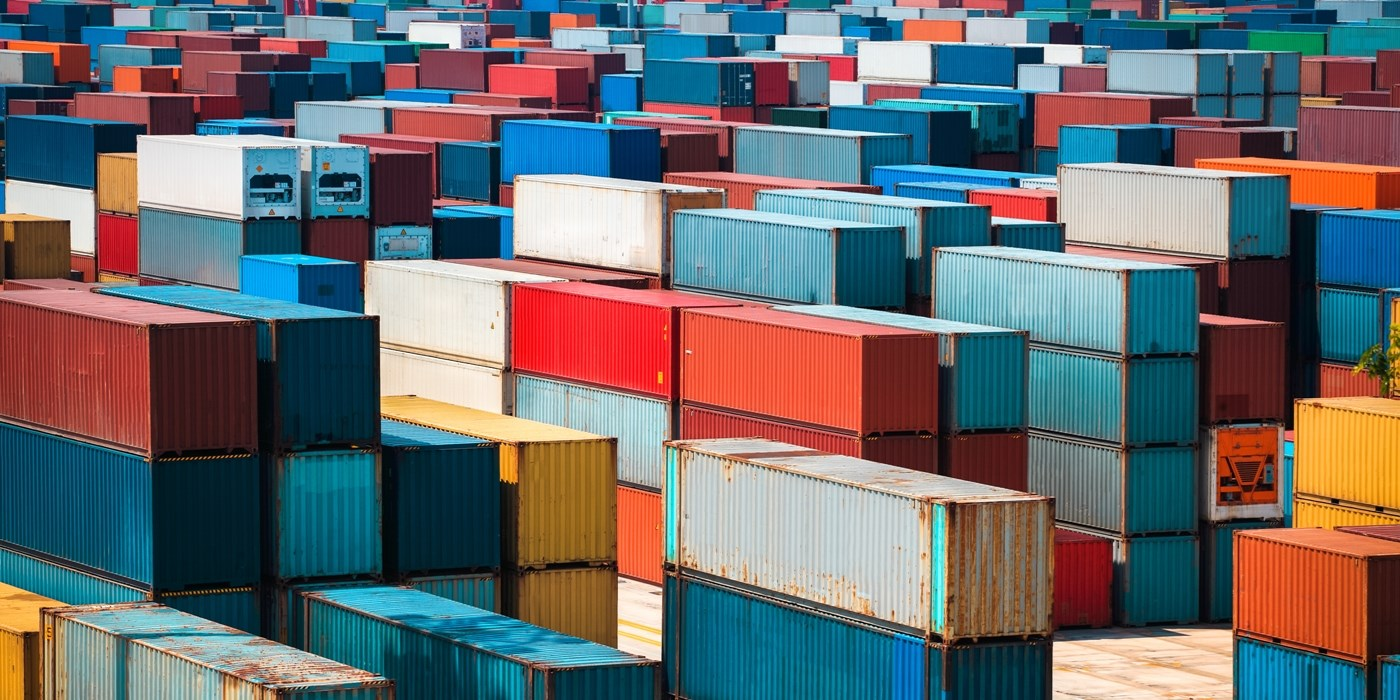
\includegraphics[height=\paperheight]{containers.jpg}
    };
    \node[minimum width=100cm, minimum height=2cm, opacity=0.75, text
          opacity=1, fill=white, at=(current page.center)]
      {\Huge Isolation};
  \end{tikzpicture}
  \vskip0pt plus 1filll
  \tiny \textcolor{white}{https://goo.gl/dqQ6lG}
\end{frame}

\begin{frame}{Scalability and Robustness}
  \smallnote{
    Mesos is a distributed system which means it has to be fast and it has to
    tolerate misbehaving clients. To improve performance, frameworks can
    install filters with the Mesos master. Each filter expresses a set of
    resources that the master shouldn't even bother offering to the framework.
    To incentivize frameworks to respond to resource offers quickly, the
    offered resources count against the framework's isolation. And to handle
    slow or crashy frameworks, Mesos can always rescind resource offers.
  }
  \begin{itemize}
    \item Frameworks can install filters with the Mesos master.
    \item Offered resources count against a framework's allocation.
    \item If a frameworks is slow to respond, Mesos can rescind offers.
  \end{itemize}
\end{frame}

\begin{frame}{Fault Tolerance}
  \smallnote{
    To handle master crashes, each Mesos master maintains soft state that is
    rederivable from slaves and frameworks. Each master also has a set of hot
    standby replicas. When a master crashes, a new leader is elected and slaves
    contact it to repopulate its soft state. To handle scheduler crashses,
    Mesos allows multiple schedulers for the same framework to be registered.
  }
  \begin{itemize}
    \item Mesos uses soft state derivable from slaves and frameworks.
    \item Hot standby replicas.
    \item Each framework can install multiple schedulers.
  \end{itemize}
\end{frame}

\begin{frame}{Placement Preferences}
  Placement preferences can be achieved with delay and lottery scheduling.
\end{frame}

\begin{frame}{Heterogenous Tasks}
  If the number of slots on each machine is big, the chances that a machine
  will be filled completely with long lived tasks is small.
\end{frame}

\end{document}
